The previous two chapters focused primarily on the performance aspects of task graph execution, by
examining various task scheduling algorithms and also bottlenecks that can limit the scalability of
existing task runtimes. Performance is naturally crucial for \gls{hpc}, yet it should
not be the only factor to focus on. \Autoref{ch:sota} discussed several other challenges
affecting \gls{hpc} task graphs, that are related to the second main focus of this
thesis, namely the \emph{ergonomics} of task graph execution.

Execution ergonomics is a broad area that encompasses several aspects, such as providing an easy
way to define the structure of the task graph, allowing its execution in an effortless manner (both
on a local computer and a distributed cluster), handling fault tolerance without the user's
intervention, allowing users to express complex resource requirements and many others. This thesis
primarily focuses on analyzing and resolving ergonomical challenges that form a barrier for
executing task graphs on \gls{hpc} clusters.

%While existing task runtimes are able to deal with some of the mentioned challenges with varying
%degrees of success, a unified, dedicated and \gls{hpc}-tailored approach for executing
%task graphs could provide added value to workflow authors, both in terms of ergonomics and
%performance.

%Apart from efficiency, there are several other important challenges have been discussed in. These
%fall under the umbrella of \emph{ergonomics} of task graph execution, which is the second
%primary focus of this thesis. Ergonomics and developer experience in general sometimes tends to be
%neglected in \gls{hpc} applications and tools, which can be notoriously difficult to
%deploy, configure and use.

%While using off-the-shelf task runtimes with \gls{hpc} clusters is possible, these
%tools are not prepared to deal with the idiosyncracies and complexities of supercomputing systems.

%Executing task graphs on \gls{hpc} clusters does not \emph{need} to be
%difficult though, if we use specialized approaches, rather than off-the-shelf tools that are not
%prepared to deal with the complexities of \gls{hpc} systems.

%Furthermore, ergonomics and performance do not
%have to contradict each other -- as we will see in this chapter, approaches that increase
%ergonomics can also help with improving performance and hardware utilization.

One approach to improve ergonomics could be to make incremental improvements to the various
mentioned challenges in off-the-shelf task runtimes. However, as we will see later in this chapter,
ergonomical areas such as supporting heterogeneous tasks and clusters and resource requirements,
providing fault tolerance and dynamic load balancing and overcoming allocation manager limits are
all intertwined, and they affect each other in non-trivial ways. Therefore, this chapter introduces
a holistic meta-scheduling design that aims to tackle the most important challenges with a unified
solution, in order to enable effortless, efficient and fault-tolerant execution of task graphs on
heterogeneous \gls{hpc} clusters in the presence of allocation managers.

This reference design has been implemented in \hyperqueue{}, an
\gls{hpc}-tailored task runtime that was designed to enable transparent, ergonomic and
efficient execution of task graphs on \gls{hpc} systems. \hyperqueue{} is a
spiritual successor of \rsds{}, and builds upon its server and task scheduler
implementation, however it does not use the \dask{} interface. It is the culmination
of the research and work presented in this thesis, which was made possible thanks to the experience
gained from \estee{} and \rsds{}, and also from interacting with many
\gls{hpc} workflows and use-cases over the course of several years.

The work presented in this chapter makes the following contributions:
\begin{enumerate}
	\item We propose a meta-scheduling design that provides a unified way of scheduling and executing tasks
	      in the presence of allocation managers and allows load balancing across different allocations. It
	      disentangles the definition of tasks and the hardware that executes them, which makes it ergonomic
	      to use.
	\item We describe an approach that enables a task runtime to automatically submit allocations on behalf
	      of the user in response to computational load, which further simplifies the execution of task
	      graphs on supercomputers.
	\item We provide a task scheduler with complex resource management that supports non-trivial features
	      that are not present in other state-of-the-art tools, such as fractional resources or resource
	      variants.
	\item We evaluate the performance and hardware utilization of the proposed design on various use-cases
	      and benchmarks.
\end{enumerate}

This chapter will first describe the general meta-scheduling design for mapping tasks to
allocations. Then we will describe the architecture of \hyperqueue{}, which implements the
proposed design. We will also provide a performance analysis of \hyperqueue{}, evaluate it
on several use-cases and compare it with other state-of-the-art meta-scheduling task runtimes.

%We have described the design and key ideas of \hyperqueue{} in
%\emph{HyperQueue: efficient and ergonomic task graphs on HPC clusters}~\cite{TODO}. The architecture of \hyperqueue{} and
%various other descriptions presented in this chapter were adapted from this publication.

\workshare{I have collaborated on this work with Ada Böhm, we have both contributed to it equally. I am the sole author of the design and implementation of
the automatic allocator component, and I have also contributed to the design and implementation of most remaining parts of
\hyperqueue{}. While me and Ada are the primary contributors to
\hyperqueue{}, it should be noted that multiple other people have contributed to it, as its development is a team effort. Source code contribution statistics for \hyperqueue{}
can be found on GitHub\footnoteurl{https://github.com/it4innovations/hyperqueue/graphs/contributors}.}

\section{Interaction with allocation managers}
The primary challenge that affects the simplicity of task graph execution on \gls{hpc}
clusters is the presence of an allocation manager, as it forms a barrier; on such clusters, it is
not possible to compute anything at all without interacting with allocations. In order for task
graph execution to become truly ergonomic, there is no point in tackling the rest of the
(ergonomical) challenges until there is a straightforward way of executing task graphs through an
allocation manager.

\Autoref{challenge:allocation-manager} has described several approaches that can be used to map tasks to
allocations, which is necessary to execute task graphs, and also their various shortcomings. Due to
the limits imposed by allocation managers, it might be necessary to partition task graphs into
multiple subgraphs in order to fit them within an allocation, which can be challenging.
Furthermore, it can result in non-optimal usage of hardware resources, because tasks from
(sub)graphs submitted in separate allocations will only be load balanced within their own
allocation, and not across different allocations.

It is important to understand what is uniquely challenging about the interaction with allocations.
The fact that the computation needs to go through a queue is not an issue by itself, as we are
dealing with batch processing anyway. Therefore, some form of a delay between submitting the task
graph and receiving the results is expected, even if we did not have to submit allocations at all.

The main issue of allocations is that they strictly tie together two separate aspects;
\emph{what} does the user want to compute (the computation performed once the allocation
starts) and \emph{where} should the computation take place (specific hardware resources
and computational nodes reserved for the allocation). As was already described previously, both of
these things have to be specified together in an allocation. This is a very inflexible design, for
several reasons:

\begin{itemize}
	\item The user needs to consider both aspects at the same time. Ultimately, the main thing that the user
	      cares about is what do they want to compute. With allocations, they also need to think about
	      specific hardware resources that should be allocated for computing their task graph, which can be
	      challenging.
	\item Hardware resources are allocated for the whole duration of the allocation. This can result in
	      inefficient resource usage, especially for heterogeneous task graphs that consist of many types of
	      tasks that use different resources. In situations where not all resources can be used at the same
	      time, some of the resources can unnecessarily sit idle. For example, consider a task graph executed
	      inside an allocation that provides two computational nodes. Tasks will be load-balanced amongst
	      these two nodes, but towards the end of the computation, there might be tasks that will take a long
	      time to finish. This might lead to a situation where only one of the nodes will be computing the
	      long tail of the remaining tasks, while the second node will be idle. Due to the fact that the
	      allocation cannot release the second node while the computation is still ongoing, the user
	      unnecessarily pays the cost of both nodes until the task graph finishes computing, even though the
	      second node is not doing any useful work.

	\item The amount of used resources has to be decided up front, new hardware resources cannot be added nor
	      removed from existing allocations. This can possibly cause inefficiencies, as described above, but
	      it also limits load balancing. If balancing only happens within (and not across) allocations, users
	      cannot easily provide new hardware resources during the computation, if they realize that it is
	      progressing too slowly.
	\item Granularity of the allocated resources might not match the granularity of tasks. Unless the
	      allocation manager supports very fine-grained allocations (e.g.\ on the level of individual
	      \gls{cpu} cores, rather than whole computational nodes), there can be a large gap
	      between the resources required by a task graph and the resources provided to an individual
	      allocation. This can again lead to resources sitting idle.
	\item Binding computation with specific hardware resources up front complicates handling of task
	      failures. When the user submits thousands of tasks on a specific set of hardware resources, and
	      some of these tasks fail, the user might need to create a new allocation to recompute the failed
	      tasks. This requires figuring out again a new set of hardware resources that should be requested,
	      as the original resources will probably not be a good fit for just a subset of the original
	      computation. A fault-tolerant design would ideally allow recomputing tasks on any compatible
	      hardware resource transparently, which goes against forcing computations and resources to be
	      defined together. Furthermore, fault tolerance should be handled automatically, without the user's
	      intervention.
\end{itemize}

It is interesting to note that some of these challenges are uniquely affecting task graphs, and in
general programming models that are different from the traditional ways of defining
\gls{hpc} computations. Consider a distributed application implemented using
\gls{mpi}, which has historically been the most common way of defining computations on
supercomputers. \gls{mpi} applications typically assume that they will run on a set of
computational nodes for a relatively long duration (hours or even days). This set of nodes
(corresponding to \gls{mpi} processes) usually does not change during the computation;
it is not trivial to add new processes, and if some of the processes crash, it typically leads to
the whole computation being aborted, as fault tolerance is not a default property of
\gls{mpi} applications~\cite{fault_tolerant_mpi}.

These properties of \gls{mpi} applications are similar to the mentioned properties of
allocations, therefore they fit together well, and using allocations to execute them is relatively
straightforward. In fact, it is clear that the allocation model itself was designed with
\gls{mpi}-like use-cases in mind. Therefore, it is not very surprising that the
concept of allocations is not a good match for programming models that are very different from
\gls{mpi}, such as task-based workflows.

%Note that several of the problems associated with using allocations are directly relevant to
%various challenges from~\Autoref{ch:sota}. Factors such as heterogeneous resource
%requirements, fault tolerance or efficient hardware usage are affected by the usage of allocations.
%Because of that, resolving the problems with allocations should also go a long way towards
%alleviating other ergonomical challenges of task graph execution.

\section{Meta-scheduling design}
This section describes a design for executing task graphs that aims to alleviate the mentioned
challenges by treating task-based programming models as first-class citizens, but still remaining
compatible with allocation managers to enable straightforward execution on \gls{hpc}
clusters. First, we will see a general overview of the design, then we will discuss its properties,
and the following sections will describe its concrete implementation within the
\hyperqueue{} task runtime.

We have seen that the most problematic aspect of allocations is the requirement to define
computations and hardware resources together. The key idea of the proposed design is thus to
completely disentangle the definition of what does the user want to compute (tasks) from the
hardware resources where the computation should take place (computational nodes,
\gls{cpu} cores, etc.). By separating these two concerns, we enable users to focus on
what they care about the most (their task graphs), instead of having to think about mapping tasks
to allocations and graph partitioning.

But how can we disentangle these two concepts when allocations require us to specify both? The
``trick'' lies in leveraging meta-scheduling on top of allocation managers, which allows us to
change what kind of computation is submitted in allocations and thus greatly simplify the
submission process. The proposed approach is built upon the following three principles.

\begin{description}[wide=0pt]
	\item[Task runtime runs outside of allocations] Moving the task runtime outside of allocations and running it at some persistent location in the
		cluster (e.g.\ on a login node) enables users to submit tasks to it in a straightforward way and
		crucially also to define the task graph independently of allocations. This removes the need to
		decide which tasks should be computed on which hardware resources and in which allocations up
		front. It can also improve hardware utilization, because it gives the task runtime the ability to
		load balance tasks across all active allocations.

		This is where the term \emph{meta-scheduling} comes in; the essence of the idea is to use a task
		runtime as a sort of high-level scheduler on top of an allocation manager. Instead of forcing users
		to think in terms of allocations, they can submit task graphs in the same way they would do it on a
		system that is not supervised by allocation managers, and let the task runtime decide in which
		allocation should a task be executed in an automatic way.

	\item[Allocations are uniform] Even if the task runtime runs outside an allocation, we still need to submit \emph{some}
		allocations to provide hardware resources that will actually execute tasks. However, instead of
		defining specific tasks that should be computed within an allocation, we can submit allocations
		that execute a generic computational provider (worker), which will connect to the task runtime
		instance running outside the allocation, and then execute tasks that are dynamically assigned to it
		by the runtime.

		With this approach, allocations become trivial and completely uniform, because they all have the
		same structure; each allocation simply starts a (set of) computational provider(s). This makes it
		much easier for users to submit allocations. Instead of thinking about how to partition their task
		graphs, users simply decide how many computational resources they want to spend at any given
		moment, and start the corresponding number of allocations. Furthermore, this also allows the task
		runtime to submit allocations completely automatically based on the current computational load.
	\item[Pair tasks with workers using abstract resources] The principles described above separate the two core pillars of task graph execution; the
		definition of the task graph and the provisioning of hardware resources. However, we actually do
		need to have \emph{some} way of tying these two aspects together, because tasks might
		have various constraints on the environment in which they can be executed. We saw that submitting
		tasks directly as allocations, which does explicitly tie tasks to a set of hardware resources, had
		many disadvantages. What we can do instead is to use a resource system that will allow us to pair
		tasks with workers in a more general and abstract way. Each task can describe a set of abstract
		resources that have to be available so that the task can be executed, and each worker will in turn
		provide a set of abstract resources that it provides. The task runtime will then dynamically assign
		tasks to workers by matching these resources together, while making sure that worker resources are
		not being oversubscribed.

		As an example, a task can specify that it requires four \gls{cpu} cores and two
		\glspl{gpu}. If we provide the task runtime with a worker that has 128 cores and 8
		\glspl{gpu}, it could schedule up to four instances of this task on this worker at the
		same time.

		This approach allows defining complex heterogeneous tasks while allowing users to provide workers
		independently of tasks, and without having to bind tasks to specific allocations.
\end{description}

The proposed design enables straightforward execution of large heterogeneous task graphs with
complex dependencies, because it sidesteps the allocation manager by moving the task runtime
outside of allocations. This avoids the limits associated with executing tasks in allocations
directly, such as limited support for dependencies, limited scale of task graphs that can be
executed, and non-optimal load balancing and hardware utilization.

This scheme can also alleviate additional challenges mentioned in~\Autoref{ch:sota}. For
example, it benefits fault tolerance, as tasks are no longer tied to specified allocations, because
they are stored in a persistent task runtime instance. When a task fails, the runtime can simply
recompute it, even in a different allocation than where it was originally started, in a way that is
fully transparent to the user. Furthermore, heterogeneous task graphs can be executed easily,
without having to consider allocation limits and the granularity of allocated hardware resources,
due to the usage of the abstract resource system. Even if the allocation manager always provides at
least a whole node in each allocation, multiple granular tasks (even from completely independent
task graphs) that require e.g.\ only a single core can be load balanced onto that same node. And
lastly, task scheduling becomes more flexible, because the task runtime can dynamically leverage
resources provided by multiple allocations at once. The last two mentioned aspects can help improve
hardware utilization in particular.

Of course, this approach is not a panacea, and it also introduces certain trade-offs. For example,
running the task runtime on a login node might be problematic if the login nodes are severely
computationally constrained or if they are not even able to connect to compute nodes of the
\gls{hpc} cluster through the network. Performance and security aspects of this
deployment method also need to be considered. In theory, the runtime could also be executed
elsewhere, for example in a cloud partition of a cluster, or even in an ephemeral way inside
allocations themselves (in that case it would still communicate with workers running in different
allocations). However, this would complicate the deployment process and it might require additional
resiliency features to be implemented in the task runtime.

To evaluate how does the proposed approach work in practice, what are its performance and usage
implications and how does it compare to existing meta-schedulers, we have implemented this design
in a task runtime called \hyperqueue{}, which will be described in the rest of this
chapter.

\section{\hyperqueue{}}
\hyperqueue{} (\hq{}) is a distributed task runtime that aims to make task graph execution a
first-class concept on supercomputers. It does that by implementing the meta-scheduling design
described in the previous section, and providing functionality optimized for \gls{hpc}
use-cases. In terms of architecture and implementation, it is an evolution of the
\rsds{} task runtime described in~\Autoref{ch:rsds}, however instead of using
the \dask{} components and \glspl{api}, it implements its own task-based
programming model. \hyperqueue{} is developed in the Rust programming language and it is
provided as an \mbox{MIT-licensed} open-source tool~\cite{hq_github}.

This section describes the high-level design of \hyperqueue{}, its programming model and
the most important features. It also presents several use-cases where it has been successfully
leveraged, and evaluates its performane and other aspects in various experiments.

%TODO: explicitly call out the challenges and how does HQ solve them?
%and also how it tackles the challenges mentioned in~\Autoref{ch:sota}.

Note that for simplicity, Slurm will be used as a default representative of an allocation manager
throughout this whole chapter, but it could be replaced by \gls{pbs} or any other
commonly used allocation manager without the loss of generality.

\subsection{Architecture}
\hyperqueue{} uses a fairly standard distributed architecture. It consists of three main
components, a central management component called a \emph{server}, a component that
serves as a computational provider which executes tasks, called a \emph{worker}, and an
interface for submitting tasks, called a \emph{client}.~\Autoref{fig:hq-architecture} displays
a high-level view of the \hq{} architecture for a typical deployment on an
\gls{hpc} cluster with an allocation manager, where the server runs on a login node
and meta-schedules tasks on top of various allocations running on computational nodes. The
individual components are described in more detail below.

\begin{figure}[h]
	\centering
	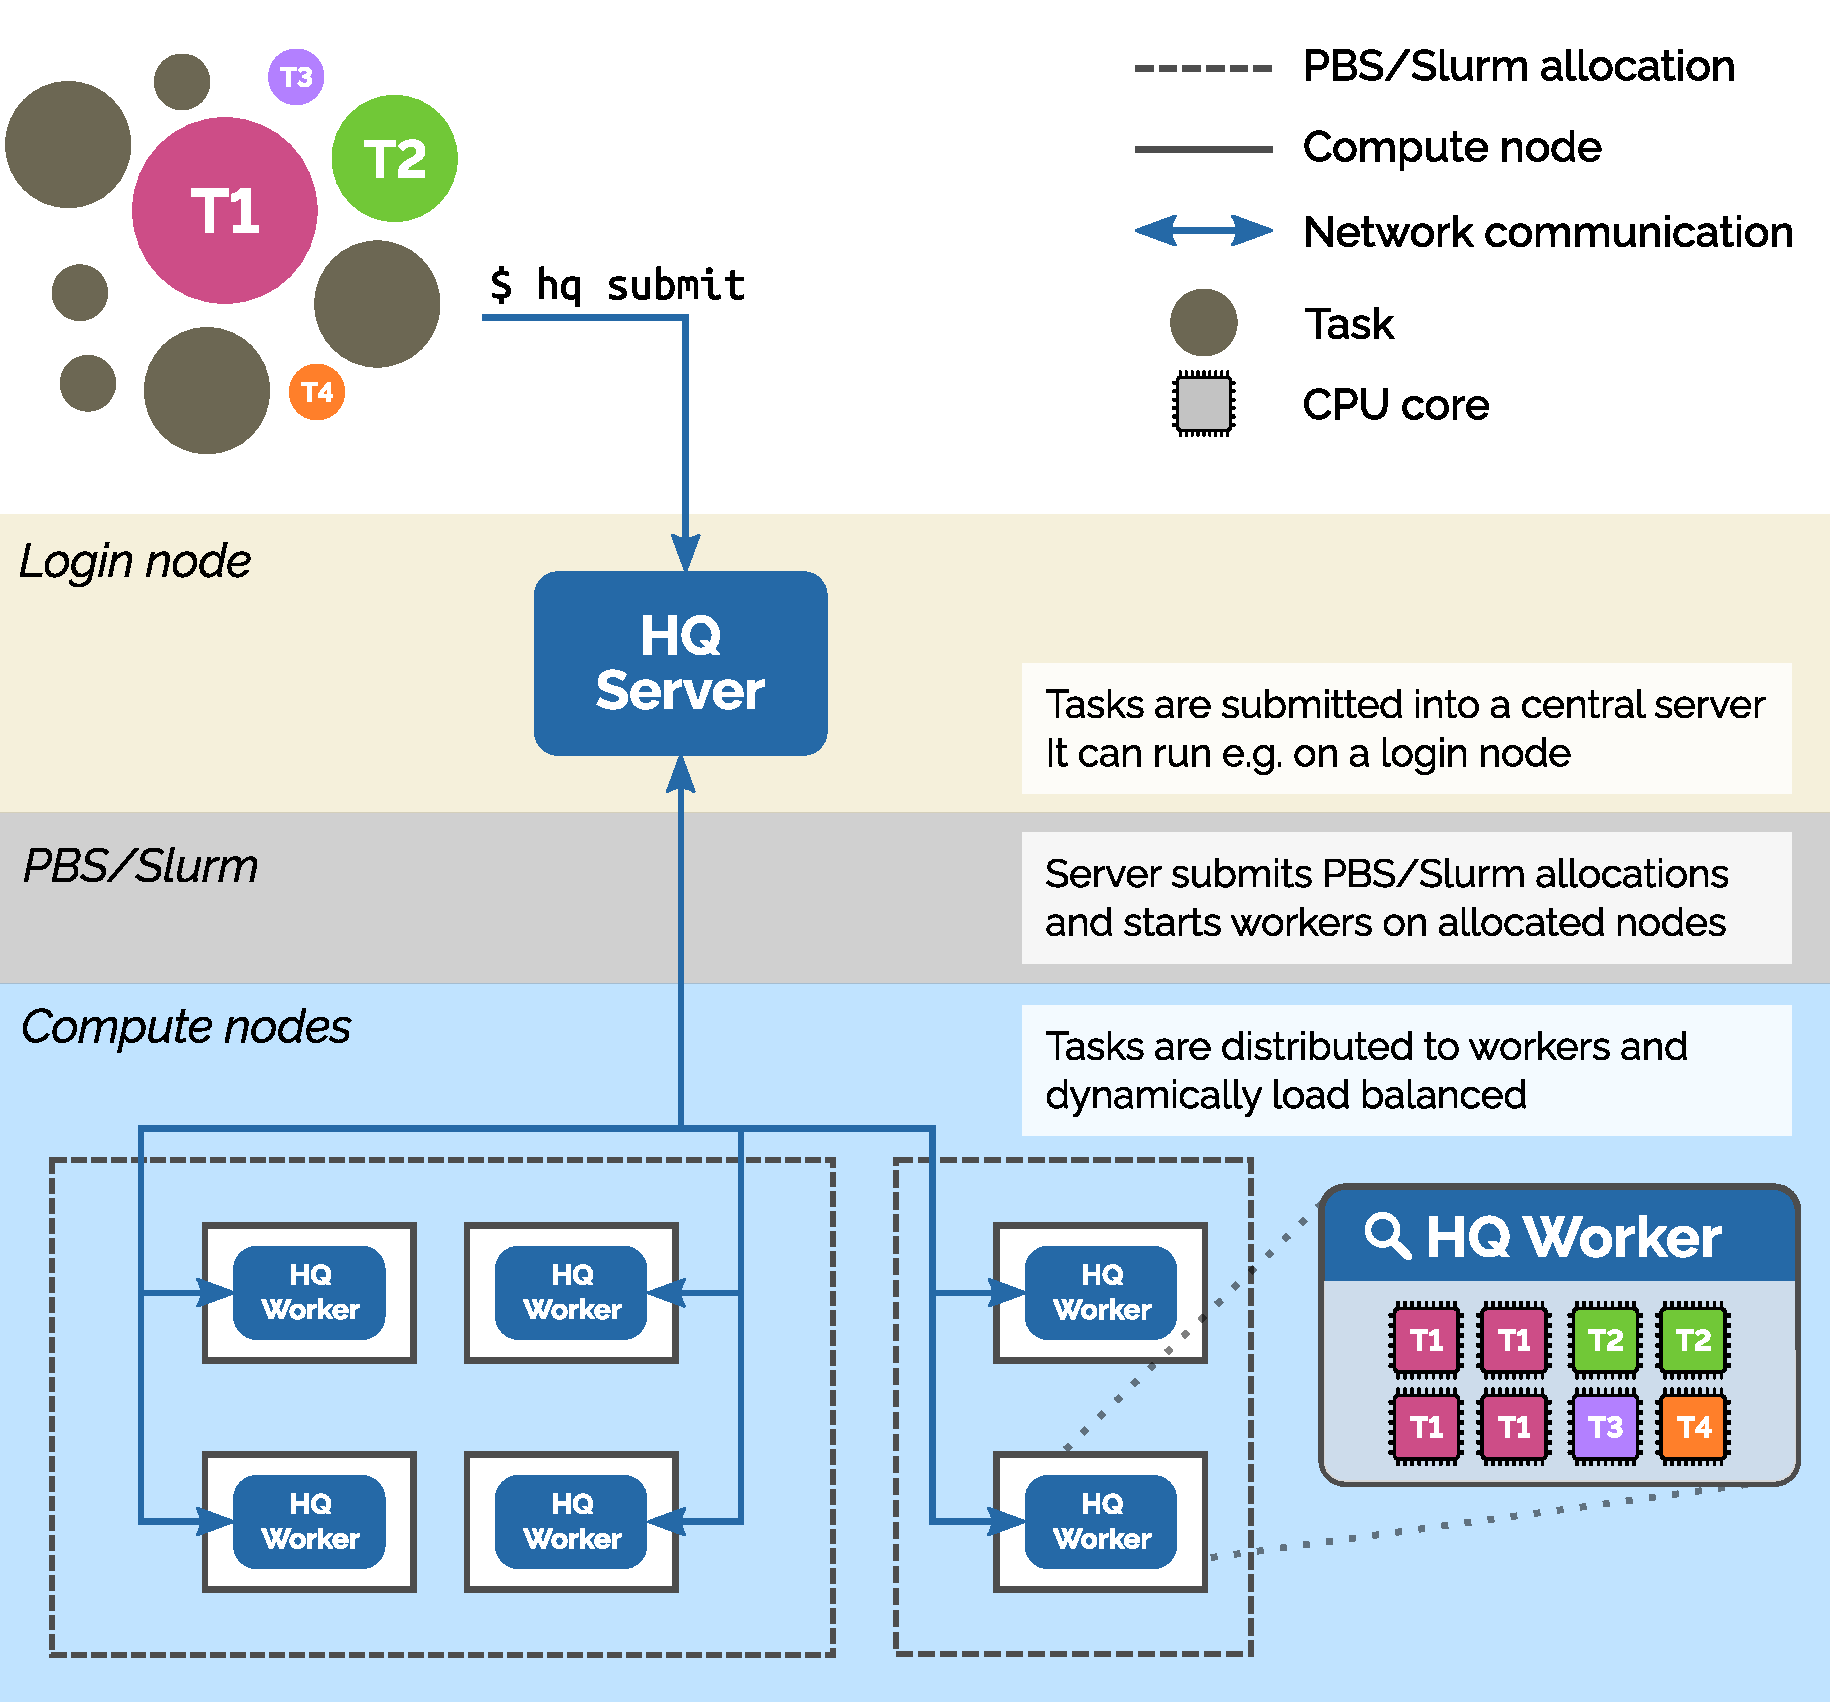
\includegraphics[width=0.9\textwidth]{imgs/hq/architecture}
	\caption{Architecture of \hyperqueue{}.}
	\label{fig:hq-architecture}
\end{figure}

\subsubsection*{Server}
The \emph{server} is the most important part of \hyperqueue{}. Its main goal is
to manage both the lifecycle of task graphs and of workers that provide computational resources. It
keeps track of all tasks and workers, and allows users to query their state and also send commands
to it through a client interface. The server contains a work-stealing task scheduler that is based
on the \rsds{} scheduler implementation described in~\Autoref{sec:rsds-description}. The
scheduler assigns individual tasks to workers based on task resource requirements and current
computational load of workers, with the goal of maximizing hardware utilization of the connected
workers.

It is designed to be executed as a long-running background process, that should ideally be executed
in a persistent location not managed by allocation managers (i.e.\ outside ephemeral allocations).
Typically, it is executed on a login node of a cluster, but it can also run elsewhere, for example
in a cloud partition. It should keep running until all tasks that the user wants to execute are
finished, although it can also restore its state from disk, so the computation of a task graph can
be interrupted and resumed at a later time, if needed.

The fact that the server runs outside allocations allows it to load balance tasks across workers
running in multiple allocations concurrently, and work around the various limits of allocation
managers. This adheres to the first principle of the meta-scheduling design described in the
previous section.

The server itself does not execute any tasks, and it consumes a relatively modest amount of
resources, therefore it is not computationally demanding. \Autoref{sec:hq-exp-server-cpu-usage} evaluates how
many \gls{cpu} resources does the server consume in extreme scenarios.

Apart from basic responsibilities related to worker management and task scheduling, the server also
provides additional functionality. For example, it can submit allocations fully automatically on
behalf of the user. This feature will be described in detail in~\Autoref{hq:automatic-allocation}.

\subsubsection*{Worker}
The \emph{worker} component is a computational provider that executes tasks assigned to
it by the server. A single worker typically manages all hardware resources (\gls{cpu}
cores, \gls{gpu} or \gls{fpga} accelerators, memory, etc.) of a given
computer, usually a single computational node of a supercomputer.

The worker is able to automatically detect all relevant hardware resources that are available on
the node where it is started and advertize them to the server. Therefore, in the typical case,
users can simply start the worker on a given node with a single uniform command, and from that
moment on the resources of that node will be used for task execution. This adheres to the second
principle of the proposed meta-scheduling design, where computational providers should be generic
(not tied to any specific task or a set of tasks), and it should be possible to start them using a
uniform command, to make their deployment trivial.

Each worker also participates in task and resource scheduling. The server makes high-level
scheduling decisions, such as which tasks will be executed on a given worker, while the worker then
performs micro decisions, such as in which order will it execute tasks assigned to it, or which
specific resources will be assigned to a given task. Resource management will be described in more
detail in~\Autoref{hq:resource-management}.

\hyperqueue{} workers were designed with fault tolerance in mind. On an \gls{hpc}
cluster, workers will be typically executed inside allocations that only run for a
limited amount of time, which implies that workers can disappear at any time during the computation
of a task graph. Both the server and workers thus operate with the assumption that workers can be
potentially short-lived and ephemeral; if a worker disconnects while it is executing a task, the
task will be transparently reassigned to a different worker without user intervention. Worker
management is thus dynamic and flexible; new workers can also be added at any time, after which
they will immeditely start contributing to the execution of the submitted task graphs. This property
enables users of \hq{} to arbitrarily scale the computation of a task graph both up and down, even
while it is being executed, by dynamically adding or removing workers as needed.

While workers can be deployed manually by users, \hq{} can also automatically
submit allocations to an allocation manager that start workers on computational nodes, based on
current computational needs of submitted task graphs, as was already mentioned. This system, called
\emph{automatic allocation}, will be described in more detail later in~\Autoref{hq:automatic-allocation}.

\subsubsection*{Client}
After starting the server, users can start submitting task graphs to it using one of several
interfaces, which implement the \emph{client} component. They can submit task graphs
either using a \gls{cli}, a \gls{toml} workflow file or using a Python
\gls{api}. The client interfaces and the programming model used by
\hq{} will be described in more detail in~\Autoref{hq:programming-model}.

\subsubsection*{Deployment}
Even though it is often overlooked, deployment of software on supercomputers can be challenging, as
was described in~\Autoref{challenge:deployment}. Since \hyperqueue{} aims to provide seamless
support for \gls{hpc} use-cases, it was also designed to be trivial to deploy. It is
distributed as a single, relatively small (approx. 15 MiB), statically linked executable, which
implements all the provided functionality (server, worker and client components). It does not
depend on any external services or dynamic libraries, apart from the ubiquitous
\texttt{C} standard library, and it runs fully in userspace and does not require any
elevated privileges. It also does not require any installation step nor any configuration.

Both clients and workers communicate with the server using the standard \gls{tcpip}
protocol, which is ubiquitously available on most clusters. By default, all communication is
encrypted, so that other users of the cluster cannot observe the data sent between the
\hyperqueue{} components. This is performed out of an abundance of caution, because the
server typically runs on a login node, which is shared by multiple users, rather than on
computational nodes, which are usually isolated between users by the allocation manager.

In order to connect the individual components using \gls{tcpip}, normally it would be
required for users to specify network hostnames and ports. While this process is relatively simple,
it still presents a minor ergonomical hurdle, because users would need to reconfigure their worker
deployment scripts and client commands every time the server would start on a new
\gls{tcpip} address. To make this easier, \hyperqueue{} removes the need to
specify hostnames and ports by default, by exploiting a useful property of \gls{hpc}
clusters, which commonly use a shared networked filesystem. When a server is created, it creates a
configuration file in the user's home directory, which contains all information necessary for
exchanging handshakes and connecting the components. When workers and clients discover the presence
of this file (which can be accessed due to the filesystem being shared), they are able to connect
to the server without the user having to specify any addresses.

Thanks to these properties, it is trivial to deploy and use \hyperqueue{} on
supercomputers, even without the involvement of the administrators of the target cluster. The
deployment benefits extend also beyond \gls{hpc} clusters. Users can also trivially
deploy \hyperqueue{} on their own personal computers. This enables them to prototype
their \gls{hpc} workflows locally, which can accelerate their development process and
is another step towards improving the ergonomics of using task graphs on supercomputers. This is in
contrast with using allocation managers for submitting tasks directly, which makes local
experimentation very difficult, as allocation managers are not straightforward to deploy on
personal computers.

%TODO: short example of CLI

\subsection{Programming model}
\label{hq:programming-model}
The task-based programming model used by \hyperqueue{} builds upon the simple task model
defined in~\Autoref{ch:taskgraphs}, while adding some additional \gls{hpc}-focused
features on top of it, such as fine-grained resource requirements and support for multi-node tasks.

The core element of the programming model is a \textbf{Task}, which has the following
properties:
\begin{itemize}
	\item It is a unit of computation. A task can be executed by \hq{}, and its execution
	      either succeeds or fails. In the current implmenetation, each task represents either the execution
	      of a binary executable, or the invocation of a single Python function, although the specific
	      details of the task execution are opaque to \hyperqueue{}.
	\item It is a unit of scheduling. The \hq{} scheduler assigns each task to a worker (or
	      to a set of workers in the case of multi-node tasks), and can work-steal tasks between workers if
	      their load is unbalanced.
	\item It forms a failure boundary. When a task fails, \hq{} can schedule it again
	      (potentially on a different worker) and restart its execution from scratch.
	\item It is a unit of dependency management. Each task may depend on a set of other tasks, and in this
	      way they may be composed in a computational \gls{dag} of tasks.
	\item It is a unit of resource management. Each task has a set of attached resource requirements, which
	      describe constraints on a computational environment where the task is allowed to be executed. The
	      \hq{} scheduler then matches these requirements with resources provided by
	      workers.
\end{itemize}

Tasks can be composed together into task graphs, which are called \textbf{Jobs} in the
\hq{} terminology. Each task belongs to exactly one job, and jobs are completely
independent, so there can be no dependencies between tasks belonging to different jobs. Jobs are
units of monitoring and management, as they allow users to group many tasks together, observe their
status or perform operations on all (or some) tasks of a job at once.

\hyperqueue{} currently does not support data transfers between tasks, as it is primarily
focused on executing tasks that execute black-box binaries which communicate through files on a
file-system. Arbitrary binary data can be attached as an input for any task, but task outputs are
only used for specifying dependencies; no task data is actually transferred between the workers.
However, this is merely a limitation of the current implementation, which we plan to lift in the
future.   %workers.%The \hq{} server is based on the \rsds{} %server, which does support data transfers between%TODO: incorporate this sentence in the above paragraph

\subsubsection{Task and job lifecycle}
The server manages the state lifecycle of tasks and jobs and also reports them to the user, so that
they can observe what is happening with their computation. At any given time, each task can be in a
single \emph{state}:

\begin{description}
	\item[Waiting] After the user creates (\emph{submits}) a task, it starts in the \emph{waiting}
		state, where it waits until it is scheduled to a worker that is able to fulfill its resource
		requirements.
	\item[Running] After a task is scheduled and starts executing on a worker, it moves on to the
		\emph{running} state. If the worker that is executing the task stops or crashes, the task
		will move back to the \emph{waiting} state, so that it can be rescheduled to a different
		worker. This is labeled as a \emph{task restart}.
	\item[Finished] When a task finishes successfully (a binary program exits with the exit code $0$
		or a Python function returns without throwing an exception), it moves to the \emph{finished}
		state.
	\item[Failed] When a task fails (a binary program exits with a non-zero exit code or a Python function throws an
		exception), it moves to the \emph{failed} state.
	\item[Canceled] When a waiting or a running task is canceled by the user, it moves to the \emph{canceled}
		state, and it is no longer considered for execution.
\end{description}

\Autoref{fig:hq-task-state-diagram} displays a state diagram of the various task states and
transitions that cause state changes. The \emph{finished}, \emph{failed} and
\emph{canceled} states are terminal; once a task reaches that state, it cannot change its
state anymore. Each job also has its associated state, which is derived from the state of its
tasks.

\begin{figure}[h]
	\centering
	\begin{tikzpicture}
		\tikzstyle{every node}=[font=\footnotesize]
		\tikzstyle{every state}=[fill={rgb:black,1;white,8},minimum size=1.5cm,font=\footnotesize]

		\node[state,initial,initial text=Submitted]   	(waiting)  							{Waiting};
		\node[state] 							   		(running) 	[right=2.5 of waiting]	{Running};
		\node[state,accepting]           		   		(finished) 	[right=2 of running]	{Finished};
		\node[state,accepting]                     		(failed) 	[above=1 of finished] 	{Failed};
		\node[state,accepting]                     		(canceled)	[below=1 of finished]   {Canceled};

		\path[->]
		(waiting)   edge [bend left]	node [above] 			{Scheduled} 		(running)
		(waiting)   edge [bend right]	node [below left]		{Canceled}			(canceled)
		(running)	edge    			node [above] 			{Finished}			(finished)
		(running) 	edge    			node [above left] 		{Failed} 			(failed)
		(running)	edge    			node [left,xshift=-5]	{Canceled} 			(canceled)
		(running)	edge [bend left]    node [below,xshift=8]	{Worker crashed}	(waiting);
	\end{tikzpicture}
	\caption{State diagram of \hyperqueue{} tasks}
	\label{fig:hq-task-state-diagram}
\end{figure}

When a worker that executes a task crashes or stops, and a task restart happens, it is important to
let the executed program know that it is not being executed for the first time, so that it can
react to it (for example clean up files that were created during a previous execution of the same
task). This is achieved using an \emph{instance ID}. It is a non-negative number attached to
each task that increases everytime the task is restarted. This number is passed to the executed
task, so that it can decide whether it should react to the restart in any specific way.

\subsection{Resource management and scheduling}
\label{hq:resource-management}
As has already been mentioned, the \hyperqueue{} scheduler is derived from the
\rsds{} work-stealing scheduler that was described in~\Autoref{sec:rsds-description}. It
assigns tasks to workers eagerly, to optimize the fast path where there are enough tasks to utilize
the available workers. When some workers are under-utilized, the server uses work-stealing to steal
tasks between workers to balance the computational load. Scheduling is performed on the level of
tasks, regardless of which job they belong to. In fact, the scheduler does not even know anything
about jobs.

What makes the scheduler different from \rsds{} is its support for complex resource
management. It takes into account various resource requirements requested by tasks, and also the
state of currently available resources on each worker, and uses this information to drive its
scheduling decisions. The most important responsibility of this resource management is to uphold
the invariant that each task will be executed on a worker that is able to provide the corresponding
amount of each resource requested by the task at the time of the task's execution. When a task is
being scheduled, the scheduler looks for a worker that can satisfy the resource requirements of the
task, based on the amount of resources provided by the worker in general, and also the amount of
resources that the worker currently has available. When a task is scheduled onto a worker, the
scheduler \emph{allocates} a specific subset of the worker's resources to that task, which
will not be available for other tasks until the scheduled tasks finished executing.

\hyperqueue{} resources are \emph{generic}, as users can define their own
arbitrary resources for both tasks and workers, although \hq{} also recognizes
several known resource names and provides specialized support for them. Resource management in
\hyperqueue{} consists of two main elements, resource requirements specified by tasks and
resource pools provided by workers.

\subsubsection*{Worker resource pools}
Worker resources are configured when a worker is started through so-called \emph{resource pools},
named sets of resources. Most common resource pools, like the \gls{cpu} cores and
\gls{numa} sockets, the amount of \gls{ram} and the presence of
\gls{gpu} accelerators, are detected automatically. On top of that, users can specify
an arbitrary set of additional pools. There are two kinds of resource pools:

\begin{description}
	\item [Indexed pool] represents a set of resources where each individual resource is
	      non-fungible and has a unique identity (represented either by an integer or a string). An example
	      of such a resource pool could be a set of \gls{cpu} cores or \gls{gpu}
	      devices. For example, if a worker has two NVIDIA \glspl{gpu}, that worker could provide
	      an indexed pool containing two resources (e.g.\ with indices $0$ and
	      $1$), each representing one individual \gls{gpu} device. These two
	      resources are not interchangeable; the scheduler decides which specific resource will be assigned
	      to a task, and it tracks the individual resources based on their identity. If a task
	      $t$ is currently using \gls{gpu} $0$, that
	      resource will not be assigned to any other task until $t$ has finished executing.

	      Individual resources of an indexed pool can be further subdivided into \emph{groups},
	      which mark some form of a relationship between specific resources. This can be used e.g.\ to
	      represent \gls{numa} domains and \gls{cpu} sockets; a worker might provide
	      a single indexed pools of \glspl{cpu}, with a separate group for each
	      \gls{numa} socket present on the worker's node. Tasks can then specify if they want to
	      prioritize drawing resources that belong to the same group, this will be described later.
	\item [Sum pool] is designed for resources that are fungible. Such resources are typically
	      numerous, and it would not be practical to track each individual resource separately. A sum pool
	      thus does not define its individual resources through indices, but only defines a single number
	      that specifies the amount of resources available in the pool. A typical representative of a sum
	      pool is \gls{ram} available on a worker. Modern \gls{hpc} nodes can
	      contain hundreds of GiBs of memory, or even more, and it is not feasible to treat each byte as a
	      separate resource. At the same time, tasks usually do not need such fine-grained tracking; if they
	      care about memory requirements, they just specify how much memory do they need.
\end{description}

%For example, the command below starts a worker that

\subsubsection*{Task resource requirements}
Resource pools define the resources that are available on workers. The scheduler then uses
\emph{resource requirements} attached to individual tasks to decide on which workers can a given task be
executed, and which specific resources it will consume while the task is running. Task resource
requirements are defined for each task separately. By default, each task requires a single
\gls{cpu} core, but users can specify a different \gls{cpu}
requirement, and also add additional arbitrary requirements.

A resource requirement consists of a name of the resource that the task needs, and an amount
specifying how many such resources are needed. For example, a task might specify that it requires
two \glspl{gpu} for its execution. The resource requirement always specifies the amount
of required resources, regardless whether the given resource is taken from an indexed or a sum
pool. Therefore, tasks cannot ask for specific instances of resources based on their identity; the
scheduler decides which specific resources will be assigned to individual tasks, which makes
scheduling more flexible. For example, assume that a worker has $128$ cores (each
with their own identity), and there is a task that requires two cores. It would not be very
practical if the task had to specify that it requires specifically cores with ID
$0$ and $1$ or $5$ and
$8$, etc. Instead, it just specifies the number of \gls{cpu} cores
it needs, and lets the scheduler decide which specific cores will it assign to the task, based on
what cores will be available on the given worker at the time the task is about to start executing.

In addition to the basic system described above, resource requirements can also leverage a few
additional parameters that allow tasks to describe more complex use-cases related to resource
management.

A \emph{group allocation strategy} can be used to affect which specific resources from an indexed pool will
be used for the task. It is not relevant for indexed pools with a single group nor for sum pools. A
typical example where indexed pool groups are useful are \gls{numa} nodes, where tasks
might want to be executed on cores that belong to the same \gls{numa} node (group). There are three
different strategies that can be selected:
\begin{description}
	\item [Compact] is the default strategy. The scheduler tries to allocate all requested
	      resources from as few groups as possible. However, if there are not enough resources currently
	      available for that on a given worker, it will also try to draw resources from a larger number of
	      groups, to satisfy the resource requirement.
	\item [Strict compact] is a stricter version of the \emph{compact} strategy. With this
	      strategy, the scheduler first figures out the minimum number of groups required to satisfy the
	      resource requirement, and it will then not schedule the task until it can provide all requested
	      resources from the smallest number of groups possible.
	\item [Scatter] is the opposite of the \emph{compact} mode. It tries to allocate resources
	      for the task from as many groups as possible.
\end{description}

Resource requirements can also be specified without an upper bound, i.e.\ a task can specify that
it wants to consume all available resources of the specified pool. If a worker has at least a
single resource of the given pool available, and the scheduler assigns a task with this kind of
resource requirement to it, that task will be allocated all the worker resources that are available
when the task starts to execute.

In some cases, requesting whole resources can still be too coarse-grained for some tasks. For
example, a task might execute software that is able to leverage \gls{gpu}
acceleration, but it cannot utilize a whole \gls{gpu} device by itself. If such task
has requested a whole \gls{gpu}, part of that accelerator's hardware might sit idle
while the task is executed. To avoid this situation, \hyperqueue{} avoid tasks to define
\emph{fractional resources}, which allow multiple tasks to share a single resource at the same time.
For example, the mentioned task could ask for only $0.5$ of a
\gls{gpu}, in which case the scheduler would allocate the same
\gls{gpu} device to up to two tasks at once. The scheduler uses fixed-point
arithmetic to manage fractional resources, in order to avoid common issues associated with
floating-point arithmetic, rounding errors.

An even more complex resource management use-case supported by \hyperqueue{} is the
ability to specify \emph{resource variants}. Normally, each resource requirement specified by a task
is additive; all the requested resources have to be available in order for the task to start
executing. However, \hq{} also allows tasks to define a list of resource
requirement sets (called resource variants), and let the scheduler use the first one that can be
satisfied by a worker at the time of scheduling (the order of the list elements decides the
priority of the individual requirement sets). Resource variants allow tasks to define multiple
situations under which it makes sense to execute the task, and let the scheduler decide which
variant to select, based on dynamic information about the current worker resource. As an example,
many \gls{hpc} software tools can run either on a \gls{cpu} or on a
\gls{gpu} device. A task using such software might specify e.g.\ that it needs either
a single \gls{gpu} and a single \gls{cpu}, or that it needs
$16$ \gls{cpu} cores (in the case that a \gls{gpu} is
not available). In this case, the scheduler could decide to execute the task purely using
\gls{cpu} resources, if there are no \gls{gpu} resources currently
available. Without support for resource variants, the scheduler would need to wait for a
\gls{gpu} to become available, even if there would be free \gls{cpu}
resources that could be used in the meantime.

There is also one additional special resource that is relevant for scheduling, called a
\emph{time request}. If a task specifies a time request (a duration) $t$, it
tells the scheduler that it needs at least $t$ time for its execution. This is
important for avoiding needless task restarts, due to the way \hq{} workers are
commonly deployed in allocations. Workers started in allocations cannot run for a longer time than
the wall-time of the allocation. Since this duration is known (each allocation must have a
wall-time), \hq{} knows the remaining lifetime of each such worker at any given
time. This information is used for scheduling; if a worker has remaining lifetime
$l$, the scheduler will not assign it tasks with a time request that is longer
than $l$, because it is highly probable that such tasks could not finish
executing before that worker would shut down.

Once a task is scheduled to a worker, and the scheduler decides which resources will be allocated
to it, it passes this information to the task through environment variables. For example, if a task
asks for two \gls{cpu} cores, and the scheduler allocated the cores
$10$ and $14$ of a specific worker to it,
\hq{} will pass \texttt{HQ\_RESOURCE\_VALUES\_cpus=10,14} to the task.

It is important to note that \hyperqueue{} treats resources as opaque and virtual; they
are used only for scheduling. \hq{} does not enforce that e.g.\ if a task is
provided the cores $0$ and $1$, it will be only executed on
these specific cores. This responsibility is left to the task itself, which can use the provided
environment variable to decide using which resources it should actually be executed. For example, a
task could pin its executed program on cores allocated to it. In the case of
\gls{cpu} cores, \hq{} can even pin the allocated cores for the
task automatically, if the task is configured for pinning.

\subsubsection*{Multi-node tasks}
\hyperqueue{} also supports a special kind of resource that is especially useful for
tasks that want to execute \gls{hpc} computations which are designed to run on
multiple nodes (e.g. \gls{mpi} programs). A task may specify that it wants to be
executed on multiple workers at the same time. In this case, \hq{} assumes
exclusive ownership of all the resources of each worker (node), which typically matches the
requirement of \gls{mpi}-like applications. A multi-node task requiring
$n$ nodes can only be scheduled when $n$ workers are idle
(not executing any tasks) at the same time. When a multi-node task starts to execute,
\hq{} passes it a \emph{nodefile} which contains the hostnames of all
workers allocated to the task. This nodefile can then be used by common \gls{mpi}
program launchers to start an \gls{mpi} program.

\subsection{Fault tolerance}
- move fault tolerance from the worker description?
- max fails

\subsection{Task submission interfaces}
The primary way of managing the \hyperqueue{} infrastructure (server and the workers) and
submitting task graphs is through a \gls{cli}, which has been designed to be familiar
to users of Slurm and \gls{pbs}. It is composed of composable subcommands that can
Unix-like philosophy.

- iterative computation?
- Python API

%\subsubsection{Output streaming}
% TODO: where to put this?

\subsection{Automatic submission of allocations}
\label{hq:automatic-allocation}
The meta-scheduling design employed by \hyperqueue{} resolves the most important
challenges associated with allocation managers, since it automates the mapping of tasks to
allocations. It also makes creating allocations simple, so that users can scale the computational
resources used for computing their task graphs at will. However, creating allocations manually can
still be relatively demanding for some users, who might want to employ a more automated approach
for scaling computational resources. Since \hyperqueue{} knows the state of all tasks and
workers, and it is commonly executed on login nodes that have access to allocation managers, it is
natural to provide it with the ability to automatically submit new allocations on behalf of the
user, based on current computational load. This system has been implemented under the name
\emph{Automatic allocator} (shortened as \emph{autoalloc}), and it will be described in this section.

The automatic allocator system in \hyperqueue{} was created with the following design
goals:
\begin{description}
	\item Allow computational resources to scale up. If there are tasks (at any given moment) that are
	      waiting to be executed, and there are no free computational resources, autoalloc should attempt to
	      add more resources by creating new allocations. At the same time, it should respect backpressure
	      from the allocation manager to avoid overloading it.
	\item Allow computational resources to scale down. Keeping allocations running on a supercomputer can be
	      quite costly. Autoalloc should thus make sure to shutdown allocations that are not performing
	      useful work because they do not have anything to compute anymore, in order to avoid wasting
	      resources.
	\item Be flexible. Allocation managers typically provide various configuration knobs that can affect the
	      behavior of allocations. While it will not ever be possible to support all possible implementations
	      of allocation managers out of the box, the automatic allocator should provide extension points that
	      enable users to configure the submitted allocations to their liking.
\end{description}

It has been implemented as a system that runs as a background service within the
\hyperqueue{} server. To use it, users first need to create at least one
\emph{allocation queue}. Such a queue describes a template for creating new allocations, which will
be submitted by \hq{} when there is a demand for more computational resources.
Each queue defines several important properties:

\begin{itemize}
	\item Time limit
	\item Backlog
	\item Worker count per allocation
	\item Max worker count
	\item Idle timeout
	\item Worker resources
	\item Custom allocation parameters
\end{itemize}

%TODO: autoalloc CLI example

- explain how backlog works
- integration with the scheduler?
- experiment with hardware utilization

\section{Case study: LiGen}
\hyperqueue{} has been used in LIGATE~\cite{ligate}.

\section{Case study: GROMACS}

\section{Related work}
\label{hq:related-work}
This section will discuss several state-of-the-art task-based tools and compare them with
\hyperqueue{}. There are hundreds of tools that are designed for executing some kind of a
task graph, whose features partially overlap with \hyperqueue{}, and it is thus
infeasible to mention all of them here.

Instead, we will focus on a smaller subset of task runtime that leverage meta-scheduling on top of
allocation managers. These tools can be more directly

Workflow management systems - more high-level - reproducibility - monitoring - cron-like

%TODO: Merlin https://merlin.readthedocs.io/en/latest/tutorial/1_introduction/?h=many#how-can-merlin-run-so-many-simulations
%TODO: Balsam https://arxiv.org/abs/1909.08704
%TODO: FireWorks https://onlinelibrary.wiley.com/doi/10.1002/cpe.3505
%TODO: Parsl
%TODO: Dask
%TODO: https://github.com/gwforg/gwf
%TODO: AutoSubmit
%TODO: https://github.com/pditommaso/awesome-pipeline

- mega-scheduling
- resources
- data transfers
- task overhead
- fault tolerance
- deployment

\section{Evaluation}
We have designed a series of experiments that evaluate the performance and scalability of
\hyperqueue{} and also its ability to maximize hardware utilization of workers. All
experiments were performed on the \gls{cpu} partition of the Karolina
supercomputer~\cite{karolina} located at the IT4Innovations supercomputing
center~\cite{it4i}. Each non-accelerated computational node of Karolina has two AMD
EPYC\texttrademark{} 7H12 2.6 GHz 64 core \glspl{cpu}, for a total of 128 cores
per node, and 256 GiB of DDR4 \gls{ram}. It runs on the RockyOS 8 operating system
with Linux kernel $4.18.0$ and \texttt{glibc} (GNU \texttt{C} standard library implementation) $2.28$.

% TODO: all experiments were performed with the 0.1X version of HyperQueue, using commit XYZ.

\subsection{Server \gls{cpu} usage}
\label{sec:hq-exp-server-cpu-usage}
The \hyperqueue{} server component is primarily designed to be executed on login nodes
when deployed on supercomputers. This could pose a problem if it consumed too many system
resources, because login nodes are shared by multiple users, and they are not designed for
computationally intensive tasks. Some clusters even forcefully limit the total amount of
\gls{cpu} time that can be consumed by processes running on login
nodes~\cite{leonardo_time_limit}, and terminate the process if it exceeds the maximum allowed time.

\begin{figure}[h]
	\centering
	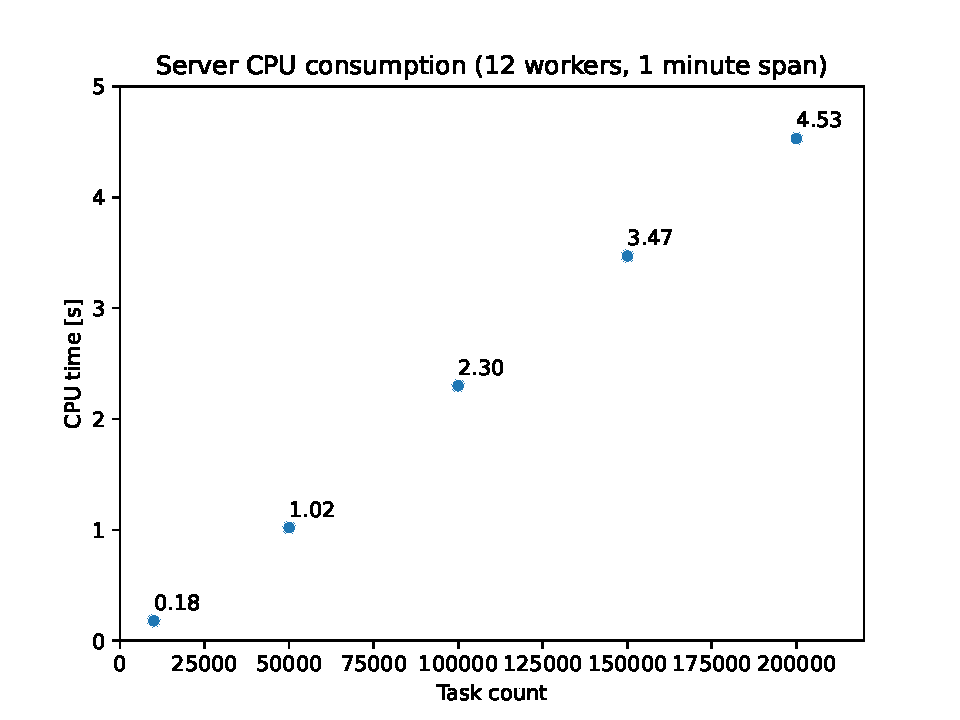
\includegraphics[width=0.7\textwidth]{imgs/hq/charts/server-utilization-tasks}
	\caption{\gls{cpu} time consumption of the \hyperqueue{} server}
	\label{fig:hq-server-cpu-consumption}
\end{figure}

To evaluate how many resources does the server consume, we have performed an experiment on the
Karolina cluster, where the server had to schedule a large number of tasks in a short time period
(which acts as a stress test), and we measured its total \gls{cpu} time consumption
across all cores.

The server was running on a login node, and it was managing $12$ workers
(therefore $1536$ cores). Each worker was deployed on a computational node in a
separate allocation, so that the server had to communicate with the workers over the network. It
had to schedule an increasing number of tasks (from $10$ to
$200$ thousand) over a fixed time span. The duration of each task was scaled so
that the whole task graph would always finish computing in exactly one minute. We measured the
total amount of \gls{cpu} time consumed by the server (both in user-space and in the
kernel), using standard Linux monitors. Each measurement was repeated five times.

We can observe the results of this experiment in~\Autoref{fig:hq-server-cpu-consumption}. The horizontal axis shows
the number of tasks that were used for the given benchmark run, and the vertical axis shows the
\gls{cpu} time consumed by the server over the one-minute period. We can see that the
amount of \gls{cpu} resources scales linearly with the number of tasks scheduled by
the server. In the worst case, the server has consumed less than five seconds of
\gls{cpu} time over one minute of real time, even though it had to schedule
$200$ thousand tasks within this short period, which is an extreme stress test
that far exceeds the rate of scheduled tasks in most scientific workflows. Over all the benchmarked
task counts, the average \gls{cpu} consumption of the server per second and per
$1000$ tasks was approximately $0.00034$~s. In other words, for every
thousand tasks in the task graph, the server consumed approximately $0.3$~ms
\gls{cpu} time every second.

In the largest evaluated case, for the task graph with $200k$ tasks, the memory
consumption of the server (measured through \gls{rss}) was approximately
$120$ MiB, which shows that the server also does not consume large amounts of
memory.

The amount of used resources will of course vary based on the executed workflow. However, this
experiment shows that the server consumes very few resources in general, and that it still has a
lot of leeway available even if some task graphs proved to be more computationally demanding than
the benchmarked stress test.

% Experiment ideas
- overhead per task of HQ vs other tools
- many sleep 0 tasks
- hardware utilization
- task storage optimization?
- time request resource waste
- encryption overhead

\section*{Summary}
This chapter has presented a meta-scheduling design designed for execution of task graphs on
\gls{hpc} clusters that was built from the ground up to overcome the issues mentioned
in\Autoref{ch:sota}. It has also introduced \hyperqueue{}, a distributed task
runtime that implements this design through an \gls{hpc} focused programming model,
which (together with its trivial deployment) makes it easy and ergonomical to run workflows on
supercomputers.  We have performed various performance evaluations% TODO: přepsat
of \hyperqueue{}, which have showed that the server does not consume a lot of resources
and that the tool as a whole is competitive with other similar tools.

%TODO: expand

As future work, we plan to add the ability to pass task outputs as inputs to dependent task, and
thus implement full data transfer functionality.

\section*{Impact}
\hyperqueue{} has already been adopted in several projects, and it is also being actively
used by various researchers and teams across several \gls{hpc} centers. It has been
proposed as one of the designated ways for executing \gls{hpc} computations in
several supercomputing centers and clusters, such as LUMI~\cite{it4i-lumi},
IT4Innovations~\cite{it4i-hq} or CINECA~\cite{cineca}.

In addition to being used directly by users as a task runtime, \hyperqueue{} can also be
integrated as a general task execution system into other tools, thanks to its sophisticated
resource management and task scheduling capabilites. It facilitates this use-case by offering a
machine-readable (\gls{json}) output mode for its \gls{cli}, which makes
it easier for other tools to use \hyperqueue{} programmatically. This has been leveraged
by several workflow management systems that have integrated \hyperqueue{} as one of their
task execution backends, such as Aiida~\cite{aiida-hq}, NextFlow~\cite{nextflow-hq},
UM-Bridge~\cite{umbridge}, StreamFlow~\cite{streamflow-hq}, ERT~\cite{ert}
or HEAppE~\cite{heappe}.

\hyperqueue{} is also being used by in various research projects. As an example,
scientists from the Czech Academy of Sciences use it to execute tasks that analyze data from the
ATLAS~\cite{atlas} experiment performed at CERN. In this case, it was able to improve
hardware utilization by 30\%~\cite{cern-hq} on the IT4Innovations \gls{hpc}
cluster. \hyperqueue{} has also been used to execute workflows in several European Union
projects, such as LIGATE~\cite{ligate}, EVEREST~\cite{everest},
ACROSS~\cite{across} and MaX~\cite{max}.

Given the use-cases mentioned above, I am confident that \hyperqueue{} provides a
tangible benefit in terms of ergonomical and efficient execution of task graphs on supercomputers,
and that it alleviates many of the challenges that have been described extensively in this thesis.
I hope that \hyperqueue{} will eventually see even more widespread usage in the
\gls{hpc} community.
